\documentclass[11pt]{article}
\usepackage[cm]{fullpage}
%%AVC PACKAGES
\usepackage{avcgreek}
\usepackage{avcfonts}
\usepackage{avcmath}
\usepackage[numberby=section,skip=9pt plus 2pt minus 7pt]{avcthm}
\usepackage{qcmacros}
\usepackage{goldstone}
%%MACROS FOR THIS DOCUMENT
\numberwithin{equation}{section}
\usepackage[
  margin=1.5cm,
  includefoot,
  footskip=30pt,
  headsep=0.2cm,headheight=1.3cm
]{geometry}
\usepackage{fancyhdr}
\pagestyle{fancy}
\fancyhf{}
\fancyhead[LE,RO]{Quiz 7, Handout 1: Perturbative analysis}
\fancyfoot[CE,CO]{\thepage}
\usepackage{url}
\makeatother
\newcommand{\resolventline}[2][1]{
  \tikz[overlay]{
      \draw[thick,flexdotted] (0,-1ex) to ++(0,#1*4.5ex) node[above,inner sep=1pt] {#2};
  }
}
\usetikzlibrary{decorations.pathreplacing}

\begin{document}


\appendix
\section{Fa\`a di Bruno's formula}

\begin{thm}
\thmtitle{Fa\`a di Bruno's formula}
\begin{align}
  \pd{^n}{x_1\cd \pt x_n}
  f(g(\bm{x}))
=
  \sum_{k=1}^n
  \sum_{(\bm{x}_1,\ld,\bm{x}_k)}^{\mc{P}_k(\bm{x})}
  f\ord{k}(g(\bm{x}))
  \prod_{i=1}^k
  \pd{
    ^{|\bm{x}_i|}
    g(\bm{x})
  }{
    x_{i,1}
  \cd
    \pt
    x_{i,|\bm{x}_i|}
  }
\end{align}
\end{thm}



\section{Direct proof of the Hausdorff expansion}

\begin{prop}\label{prop:nested-commutator}
\thmtitle{Nested commutator relation}
\thmstatement{
$\ds{
  [X,\,\cdot\,]^n(Y)
=
  \sum_{k=0}^n
  (-)^k
  {n\choose k}
  X^{n-k}YX^k
}$.
}
\thmproof{
We proceed by induction on $n$.
For $n=1$ this follows from the definition of the commutator,
$
  [X,Y]
=
  XY
-
  YX
$.
Assuming the proposition holds for $n-1$ nested commutators, we can express the $n$-fold nested commutator as
\begin{align*}
  [X,\,\cdot\,]^n(Y)
=
  X[X,\,\cdot\,]^{n-1}(Y)
-
  [X,\,\cdot\,]^{n-1}(Y)\,X
=
  X^kY
+
  \sum_{k=1}^{n-1}
  (-)^k
  \pr{
    {n-1\choose k}
  +
    {n-1\choose k-1}
  }
  X^{n-k}YX^k
+
  (-)^nYX^n
\end{align*}
by expanding $[X,\,\cdot\,]^{n-1}(Y)$ twice and substituting $k$ for $k-1$ in the second summation.
Combining factorials as follows
\begin{align*}
  {n-1\choose k}
+
  {n-1\choose k-1}
=
  \fr{n-k}{n-k}\cdot
  \fr{(n-1)!}{k!(n-1-k)!}
+
  \fr{k}{k}\cdot
  \fr{(n-1)!}{(k-1)!(n-k)!}
=
  {n\choose k}
\end{align*}
shows that the proposition also holds for $n$, completing the proof by induction. 
}
\end{prop}

\begin{thm}\label{thm:hausdorff}
\thmtitle{The Hausdorff Expansion}
\thmstatement{
$\ds{
  e^{X}Ye^{-X}
=
  \sum_{n=0}^\infty
  \fr{1}{n!}
  [X,\,\cdot\,]^n(Y)
}$
}\vspace{5pt}
\thmproof{
This follows from a direct Taylor expansion of the exponentials, along with proposition~\ref{prop:nested-commutator}.\footnote{For a slick alternative to this proof, see Helgaker, J\o rgensen, and Olsen, \textit{Molecular Electronic-Structure Theory} (2000), p.~100.}
\begin{align*}
  e^XYe^{-X}
=
  \sum_{h=0}^\infty
  \sum_{k=0}^\infty
  \fr{1}{h!\,k!}
  (-)^k
  X^hYX^k
=
  \sum_{n=0}^\infty
  \fr{1}{n!}
  \sum_{k=0}^n
  \fr{n!}{(n-k)!\,k!}
  (-)^k
  X^{n-k}
  Y
  X^k
=
  \sum_{n=0}^\infty
  \fr{1}{n!}
  [X,\,\cdot\,](Y)
\end{align*}
In the second step, we have rearranged the sum to run over $n=h+k$ and $k$ and inserted
$
  1
=
  n!/n!
$.
}
\end{thm}



\section{L\"owdin partitioning matrix derivation}


\begin{rmk}
\label{rmk:lowdin-partitioning}
\thmtitle{L\"owdin partitioning}
For a given truncation level $m$, let us refer to the span of
$\bm{\F}_\mr{i}=\pma{\F\ \bm{\F}_1\,\cd\,\bm{\F}_m}$
as the
\textit{internal space}
and that of
$\bm{\F}_\mr{e}=\pma{\bm{\F}_{m+1}\,\cd\,\bm{\F}_n}$
as the
\textit{external space}, so that
$
  \kt{\bo{\F}_\mr{i}}
  \br{\bo{\F}_\mr{i}}
+
  \kt{\bo{\F}_\mr{e}}
  \br{\bo{\F}_\mr{e}}
=
  1_n
$.
In the coordinate space over $\bo{\F}$ this reads
$
  \bo{1}_\mr{i}
+
  \bo{1}_\mr{e}
=
  \bo{1}
$,
in terms of the following projection matrices.
\begin{align}
  \bo{1}_\mr{i}
\equiv
  \ip{\bo{\F}|\bo{\F}_\mr{i}}
  \ip{\bo{\F}_\mr{i}|\bo{\F}}
=
\pma[l]{
  \bo{1} & \bo{0} \\
  \bo{0} & \bo{0}
}
&&
  \bo{1}_\mr{e}
\equiv
  \ip{\bo{\F}|\bo{\F}_\mr{e}}
  \ip{\bo{\F}_\mr{e}|\bo{\F}}
=
\pma[l]{
  \bo{0} & \bo{0} \\
  \bo{0} & \bo{1}
}
\end{align}
This allows us to write vector decompositions as
$
  \bo{c}
=
  \bo{c}_\mr{i}
+
  \bo{c}_\mr{e}
$
and matrix decompositions as
$
  \bo{H}
=
  \bo{H}_\mr{ii}
+
  \bo{H}_\mr{ie}
+
  \bo{H}_\mr{ei}
+
  \bo{H}_\mr{ee}
$
in terms of
$
  \bo{c}_\mr{x}
\equiv
  \bo{1}_\mr{x}\,
  \bo{c}
$
and
$
  \bo{H}_\mr{xy}
\equiv
  \bo{1}_\mr{x}\,
  \bo{H}\,
  \bo{1}_\mr{y}
$.\footnote{Note that I am dropping the subscript $e$ on the Hamiltonian and energy here to avoid confusion with $\mr{e}$.}
Finally, note that the \textit{external space resolvent}
$
  \bo{R}_\mr{ee}
\equiv
\left.
  (
    E
  -
    \bo{H}
  )^{-1}
\right|_\mr{e}
$
satisfies
\begin{align}
  \bo{R}_\mr{ee}\,
  (
    E
  -
    \bo{H}
  )
=
-
  \bo{R}_\mr{ee}\,
  \bo{H}_\mr{ei}
+
  \bo{1}_\mr{e}
&&
  (
    E
  -
    \bo{H}
  )\,
  \bo{R}_\mr{ee}
=
-
  \bo{H}_\mr{ie}\,
  \bo{R}_\mr{ee}
+
  \bo{1}_\mr{e}
\end{align}
and operating the left equation on $\bo{c}$ gives zero due to the Schr\"odinger equation, implying that
$
  \bo{c}_\mr{e}
=
  \bo{R}_\mr{ee}
  \bo{H}_\mr{ei}
  \bo{c}_\mr{i}
$.
Projecting the Schr\"odinger equation by $\bo{1}_\mr{i}$ and substituting in this expression for $\bo{c}_\mr{e}$ then leads to
\begin{align}
  (
    \bo{H}_\mr{ii}
  +
    \bo{V}_\mr{ii}
  )
  \bo{c}_\mr{i}
=
  E
  \bo{c}_\mr{i}
&&
  \bo{V}_\mr{ii}
\equiv
  \bo{H}_\mr{ie}
  \bo{R}_\mr{ee}
  \bo{H}_\mr{ei}
\end{align}
which reduces the Schr\"odinger equation on $\mc{F}_n$ to an effective Schr\"odinger equation in the internal space.
This gives
\begin{align}
\label{eq:lowdin-functional}
  E
=
  \fr{
    \bo{c}_\mr{i}\dg
    (
      \bo{H}_\mr{ii}
    +
      \bo{V}_\mr{ii}
    )
    \bo{c}_\mr{i}
  }{
    \bo{c}_\mr{i}^*\cdot
    \bo{c}_\mr{i}
  }
\end{align}
which expresses the exact energy in terms of internal-space coefficients.
Let us refer to this energy expression as the \textit{L\"owdin functional}.
The L\"owdin functional is the central equation in the \textit{L\"owdin partitioning} method, which can be used to eliminate the leading error incurred by truncating at a given excitation level $m<n$.
\end{rmk}


\section{L\"owdin partitioning for CI}


\begin{rmk}
$
  \Y_\mr{i}\bord{\ceil{m/2}}
=
  \Y_{\mr{CIS}{\cd}m}
$
and
$
(
  E
-
  H
)\ord{0}
=
-
  H_0
$
\begin{align}
  E
-
  E_{\mr{CIS}{\cd}m}
\approx
  \ip{\Y_{\mr{CIS}{\cd}m}|V_\mr{c}|\bo{\F}_\mr{e}}
  \ip{\bo{\F}_\mr{e}|E_\mr{c} - H_\mr{c}|\bo{\F}_\mr{e}}^{-1}
  \ip{\bo{\F}_\mr{e}|V_\mr{c}|\Y_{\mr{CIS}{\cd}m}}
\end{align}
\begin{align}
  E
-
  E_{\mr{CIS}{\cd}m}
=
  (\tfr{1}{(m+1)!})^2
  \sum_{\substack{a_1\cd a_{m+1}\\i_1\cd i_{m+1}}}
  \fr{
    |\ip{\F_{i_1\cd i_{m+1}}^{a_1\cd a_{m+1}}|V_\mr{c}\,(C_{m-1} + C_m)|\F}|^2
  }{
    \mc{E}_{a_1\cd a_{m+1}}^{i_1\cd i_{m+1}}
  }
+
  (\tfr{1}{(m+2)!})^2
  \sum_{\substack{a_1\cd a_{m+2}\\i_1\cd i_{m+2}}}
  \fr{
    |\ip{\F_{i_1\cd i_{m+2}}^{a_1\cd a_{m+2}}|V_\mr{c}\,C_m|\F}|^2
  }{
    \mc{E}_{a_1\cd a_{m+2}}^{i_1\cd i_{m+2}}
  }
\end{align}
\end{rmk}



\section{EOM-CC matrix equations}


\begin{rmk}
Note that the EOM-CC equations can be expressed in matrix notation as
\begin{align}
\label{eq:eom-matrix-equations}
  \ol{\bo{H}}
  \bo{r}_k
=
  E_k
  \bo{r}_k
&&
  \bo{l}_k\dg
  \ol{\bo{H}}
=
  \bo{l}_k\dg
  E_k
&&
  \bo{l}_k^*\cdot
  \bo{r}_l
=
  \d_{kl}
&&
  \ol{\bo{H}}
=
\pma{
  E
&
  \ip{\F|\ol{H}|\bo{\F}_1}
&
  \ip{\F|\ol{H}|\bo{\F}_2}
&
  \cd
\\
  0
&
  \ip{\bm{\F}_1|\ol{H}|\bo{\F}_1}
&
  \ip{\bm{\F}_1|\ol{H}|\bo{\F}_2}
&
  \cd
\\
  0
&
  \ip{\bm{\F}_2|\ol{H}|\bo{\F}_1}
&
  \ip{\bm{\F}_2|\ol{H}|\bo{\F}_2}
&
  \cd
\\
  \vd
&
  \vd
&
  \vd
&
  \dd
}
\end{align}
where we can identify the ground-state right eigenvector by inspection as $\bo{r}_0=\ip{\bo{\F}|\F}$ with eigenvalue $E$.
\end{rmk}




\newpage
\section{Frantz-Mills factorization theorem}

\begin{dfn}
\label{dfn:level}
\thmtitle{Level}
Products of operators and resolvents are represented by graphs with resolvent lines.
When each resolvent line spans the width of the diagram, we can partition a graph's operators into distinct \textit{levels} numbered from bottom to top with zero indexing.
An operator lies in the $k\eth$ level if there are $k$ resolvent lines below it.
A line originating in the $k\eth$ level and terminating in the $k'{}\eth$ level crosses the $i\eth$ resolvent line if $\mr{min}(k,k')<i\leq \mr{max}(k,k')$.
\end{dfn}

\begin{dfn}
\label{dfn:resolvent-graph}
\thmtitle{Resolvent graph}
A \textit{resolvent graph} $R\equiv(G,m,\rh)$ partitions $G$'s operators into $m$ distinct levels, placing the operator $o$ in level $\rh(o)\in\mb{Z}_m$ through the \textit{level map}, $\rh$.\,\footnote{
  $\mb{Z}_m$ denotes the first $m$ nonnegative integers,
  $
  \{
    0,1,\ld,m-1
  \}
  $.
  Note that an $m$-level resolvent graph contains $m-1$ resolvents.
}
\end{dfn}

\begin{dfn}
\thmtitle{Substitution}
Let $G[H\mapsto o\,]$ denote the \textit{substitution} of a connected subgraph $H$ in $G$ with an operator $o$ containing the same number of open cycles.
An analogous operation,
$
  R[S\mapsto o\,]
$,
can be performed for resolvent graphs.
Let
$
  R_k
=
(
  G_k,
  \rh_k,
  k+2
)
$
denote the substitution of everything above the $k\eth$ resolvent line in $R$ by a single operator, $\widetilde{o}_{k+1}$.
\end{dfn}

\begin{rmk}
A product of graphs $G=(L,O,h,t)$ and $G'=(L',O',h',t')$ forms a new graph given by
\begin{align}
  GG'
=
  (L\cup L', O\cup O', h\oplus h', t\oplus t')
\end{align}
where $h\oplus h'$ acts as $h$ on lines from $L$ and as $h'$ on lines from $L'$.
The combined tail function is defined similarly.
\end{rmk}


\begin{dfn}
\label{dfn:zipper-graph}
\thmtitle{Zipper graph}
A \textit{zipper graph} $(RR')_\pi^{k,k'}$ joins $R$ and $R'$ at levels $k$ and $k'$ and interleaves their lower levels with a riffle-shuffle
$\pi\in\mr{S}_{\mb{Z}_{k+k'}}^{(k,k')}$.
Formally, the zipper graph is defined as follows, in terms of $R_k$ and $R_{k'}'$.
\vspace{-10pt}
\begin{align*}
  (RR')_\pi^{k,k'}
\equiv
(
  G_k
  G_{k'}',\, 
  k+k'+2,\,
  \rh_\pi^{k,k'}
)
&&
\begin{array}{l@{\,}lc}
    \rh_\pi^{k,k'}
    (o')
&
  =
  \left\{
  \begin{array}{ll}
    \rh_{k'}'(o') + k
  &
    \makebox[3em][r]{$\rh_{k'}'(o')$}
  \geq
    k'
  \\
    \makebox[2.1cm][l]{$\pi(\rh_{k'}'(o')+k)$}
  &
    \makebox[3em][r]{$\rh_{k'}'(o')$}
  <
    k'
  \end{array}
  \right.
&
  o'
\in
  O'
\\[10pt]
    \rh_\pi^{k,k'}
    (o\,)
&
  =
  \left\{
  \begin{array}{ll}
    \rh_k(o) + k'
  &
    \makebox[3em][r]{$\rh_k(o)$}
  \geq
    k
  \\
    \makebox[2.1cm][l]{$\pi(\rh_k(o))$}
  &
    \makebox[3em][r]{$\rh_k(o)$}
  <
    k
  \end{array}
  \right.
&
  o
\in
  O
\end{array}
&&
&&
\begin{tikzpicture}[baseline=-2.5pt,inner sep=0pt]
  \node[inner sep=0pt] {
    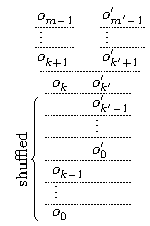
\includegraphics[width=2.7cm]{figs//zipper-graph.pdf}
  };
\end{tikzpicture}
\end{align*}
The diagram on the right displays the structure of a zipper graph, assuming that $R$ and $R'$ have one operator per level.
The two subgraphs above the combined level correspond to $\widetilde{o}_{k+1}$ and $\widetilde{o}'_{k'+1}$ in $R_k$ and $R_{k'}'$.
\end{dfn}

\begin{thm}
\label{thm:frantz-mills-factorization}
\thmtitle{The Frantz-Mills factorization theorem}
\thmstatement{
$\displaystyle{
  RR'
=
  \sum_\pi
  (RR')_\pi^{k,k'}
}$
}
\thmproof{
}
\end{thm}



\begin{dfn}
\label{dfn:insertion-graph}
\thmtitle{Insertion graph}
\end{dfn}


%\begin{dfn}
%\thmtitle{Insertion graph}
%The graphs encountered in perturbation theory contain operators separated by resolvents.
%Two disconnected parts are termed \textit{separate} if no resolvent line crosses both.
%Vertical spaces between resolvent lines are termed \textit{levels}, which we number from %top to bottom for each separate part.
%A pair of resolvents with no intervening operators encloses an \textit{empty level}.
%Inserted brackets in the bracketing expansion produce separate and unlinked \textit{insertion graphs}.
%The empty level in the \textit{remainder} created by the insertion is the \textit{level of the insertion}.
%\end{dfn}


\newpage
\section{Orbital optimization}


\begin{align}
  H
=
  h_p^q
  a^p_q
+
  \tfr{1}{4}
  \ol{g}_{pq}^{rs}
  a^{pq}_{rs}
\end{align}

\begin{align}
  E
=
  h_p^q
  \g^p_q
+
  \tfr{1}{4}
  \ol{g}_{pq}^{rs}
  \g^{pq}_{rs}
\end{align}

\begin{align}
  \mc{L}
=
  \mr{Re}
  (
    h_p^q
    \ol{\g}^p_q
  +
    \tfr{1}{4}
    \ol{g}_{pq}^{rs}
    \ol{\g}^{pq}_{rs}
  )
&&
\begin{array}{r@{\ }l}
  \ol{\g}^p_q
&\equiv
  \ip{\F|(1+\La)\,a^p_q\,\mr{exp}(T)|\F}_\mr{C}
\\[4pt]
  \ol{\g}^{pq}_{rs}
&\equiv
  \ip{\F|(1+\La)\,a^{pq}_{rs}\,\mr{exp}(T)|\F}_\mr{C}
\end{array}
\end{align}

\begin{align}
  \mc{L}
=
  h_p^q
  \g^p_q
+
  \tfr{1}{4}
  \ol{g}_{pq}^{rs}
  \g^{pq}_{rs}
&&
\begin{array}{r@{\ }l}
  \g^p_q
&\equiv
  \tfr{1}{2}
  (
    \ol{\g}^p_q
  +
    \ol{\g}^{q*}_p
  )
\\[4pt]
  \g^{pq}_{rs}
&\equiv
  \tfr{1}{2}
  (
    \ol{\g}^{pq}_{rs}
  +
    \ol{\g}^{rs*}_{pq}
  )
\end{array}
\end{align}


\section{ROHF}

Let $\bm\f_\mr{d}$, $\bm\f_\mr{s}$, and $\bm\f_\mr{v}$ be column vectors of doubly occupied, singly occupied, and virtual orbitals.
Each of these spatial functions corresponds to two spin-orbital vectors, $\bm{\f}_\mr{x}\a$ and $\bm{\f}_\mr{x}\b$, and the SODS-ROHF effective Fock operator is given (in the Guest-Saunders approach) by the following
\begin{align}
  \op{f}_\mr{eff}
\equiv
  \ma{
    \op{1}_\mr{d} &
    \op{1}_\mr{s} &
    \op{1}_\mr{v}
  }
  \ma{
    \op{f}_\mr{avg} & \op{f}_\b       &  \op{f}_\mr{avg} \\
    \op{f}_\b       & \op{f}_\mr{avg} &  \op{f}_\a       \\
    \op{f}_\mr{avg} & \op{f}_\a       &  \op{f}_\mr{avg} \\
  }
  \ma{
    \op{1}_\mr{d} \\
    \op{1}_\mr{s} \\
    \op{1}_\mr{v} \\
  }
&&
  \op{f}_\mr{avg}
\equiv
  \tfr{1}{2}
  (
    \op{f}_\a
  +
    \op{f}_\b
  )
&&
  \op{1}_\mr{x}
\equiv
  \kt{\bm\y_\mr{x}}
  \br{\bm\y_\mr{x}}
\end{align}
where $\op{f}_\a$ and $\op{f}_\b$ are the usual Fock operators, defined in terms of $\op{f}_\mr{eff}$'s self-consistent densities.


Start with the canonical Hartree-Fock equation
\begin{align}
  \op{f}_\mr{eff}
  \f_p
=
  \ev_p
  \f_p
&&
  \op{f}_\mr{eff}
=
  \sum_{\mr{x},\mr{y}}
  \op{1}_\mr{x}
  \,
  \op{f}_\mr{eff}^{\mr{x},\mr{y}}
  \,
  \op{1}_\mr{y}
\end{align}
and expand it in the AO basis.
\begin{align}
  \ip{\bm\x|\op{f}_\mr{eff}|\bm\x}
  \bo{c}_p
=
  \ev_p
  \ip{\bm\x|\bm\x}
  \bo{c}_p
&&
  \op{1}_\mr{x}
=
  \kt{\bm\f_\mr{x}}
  \br{\bm\f_\mr{x}}
=
  \kt{\bm\x}
  \bo{C}_\mr{x}
  \bo{C}_\mr{x}\dg
  \br{\bm\x}
\end{align}
Yields the following
\begin{align}
  \ip{\bm\x|\op{f}_\mr{eff}|\bm\x}
=
  \sum_{\mr{x},\mr{y}}
  \bo{P}_\mr{x}\dg
  \ip{\bm\x|\op{f}_\mr{eff}^\mr{x,y}|\bm\x}
  \bo{P}_\mr{y}
&&
  \bo{P}_\mr{x}
\equiv
  \bo{C}_\mr{x}\bo{C}_\mr{x}\dg
  \ip{\bm\x|\bm\x}
\end{align}
designating the single occupations as alpha spins, we have the following relationships
\begin{align}
  \bo{P}_\mr{d}
=
  \bo{D}_\b\bo{S}
&&
  \bo{P}_\mr{s+d}
=
  \bo{D}_\a\bo{S}
&&
  \op{1}_\mr{s}
=
  \op{1}
-
  \op{1}_\mr{d}
&&
  \op{1}_\mr{v}
=
  \op{1}
-
  \op{1}_\mr{s+d}
\end{align}
where
$
  \bo{D}_\b
=
  \bo{C}_{\mr{o}_\b}
  \bo{C}_{\mr{o}_\b}\dg
$
and
$
  \bo{D}_\a
=
  \bo{C}_{\mr{o}_\a}
  \bo{C}_{\mr{o}_\a}\dg
$
are the UHF density matrices.
This allows us to express the AO-basis pseudo-projection operators as follows.
\begin{align}
  \bo{P}_\mr{d}
=
  \bo{D}_\b
  \bo{S}
&&
  \bo{P}_\mr{s}
=
  (\bo{D}_\a - \bo{D}_\b)
  \bo{S}
&&
  \bo{P}_\mr{v}
=
  \bo{1}
-
  \bo{D}_\a
  \bo{S}
\end{align}
The final expression for the effective Fock matrix in terms of UHF Fock matrices is as follows.
\begin{align}
  \bo{F}_\mr{eff}
=
  \tfr{1}{2}
  \sum_{
    \substack{
      \mr{x},\mr{y}\in\{\mr{d},\mr{v}\} \\
      \mr{x} = \mr{y} = \mr{s}
    }
  }
  \bo{P}_\mr{x}\dg
  (\bo{F}_\a + \bo{F}_\b)
  \bo{P}_\mr{y}
+
  \sum_{\mr{x}\neq\mr{y}\in\{\mr{d},\mr{s}\}}
  \bo{P}_\mr{x}
  \bo{F}_\b
  \bo{P}_\mr{y}
+
  \sum_{\mr{x}\neq\mr{y}\in\{\mr{s},\mr{v}\}}
  \bo{P}_\mr{x}
  \bo{F}_\a
  \bo{P}_\mr{y}
\end{align}

\end{document}
